\documentclass[../thesis]{subfiles}
\begin{document}

\chapter{Hardware emulation investigation\label{chap:hardware}}
In order to experiment with integrating CHERI and RVV, we implemented a RISC-V emulator in the Rust programming language named \code{riscv-v-lite}.
The emulator can partially emulate four unprivileged\footnote{i.e. entirely bare-metal without privilege levels for OSs or hypervisors.} RISC-V ISAs (\cref{tab:emu_arches}), and was also used as the base for capabilities-in-vectors research (\cref{chap:capinvec}).
This chapter explores the development of the emulator, the implementation of CHERI support (including supplementary libraries), the addition of vector support, and the conclusions drawn about CHERI-RVV.

\begin{table}[h]
    \centering
    \begin{tabular}{cll}
    \toprule
    \multicolumn{2}{c}{Architecture} & Extensions \\
    \midrule
    32-bit & \code{rv32imv} & Multiply, CSR, Vector\parnote{Floating-point parts of the vector extension are not supported.\label{rvvnofloat}}  \\
    64-bit & \code{rv64imv} & Multiply, CSR, Vector\parnoteref{rvvnofloat}  \\
    64-bit & \code{rv64imvxcheri} & Multiply, CSR, Vector\parnoteref{rvvnofloat}, CHERI  \\
    64-bit & \code{rv64imvxcheri-int} & Multiply, CSR, Vector\parnoteref{rvvnofloat}, CHERI (Integer)  \\
    \bottomrule
    \end{tabular}
    \parnotes
    \caption{\code{riscv-v-lite} supported architectures}\label{tab:emu_arches}
\end{table}

\section{Developing the emulator}\label{chap:software:sec:emu}

Each architecture is simulated in the same way.
A \code{Processor} struct holds the register file and memory, and a separate \code{ProcessorModules} struct holds the ISA modules the architecture can use.
% A separate \code{ProcessorModules} struct holds all ISA modules the processor can execute (e.g. the base RV64 Integer ISA, the Multiply extension, and the Vector extension).
Each ISA module uses a ``connector'' struct to manipulate data in the \code{Processor}.
% The gap between the \code{Processor} and the ISA modules is bridged by a module-specific ``connector'' struct, which holds references to data in the \code{Processor} that is required by the ISA module.
For example, the RV64 Integer ISA's connector contains the current PC, a virtual reference to a register file, and a virtual reference to memory.
This allows different \code{Processor} structs (e.g. a normal RV64 and a CHERI-enabled RV64) to reuse the same ISA modules despite using different register file implementations.

Each \code{Processor} implements a single stage pipeline.
Instructions are fetched, decoded with a common decoder function\footnote{The decoder, and therefore all emulated processors, doesn't support RISC-V Compressed instructions.}, and executed.
The processor asks each ISA module in turn if it wants to handle the instruction, and uses the first module to say yes.
If the ISA module returns a new PC value it is immediately applied, otherwise it is automatically incremented.
This structure easily represents basic RISC-V architectures, and can scale up to support many different new modules.

\subsection{Emulating CHERI}

Manipulating CHERI capabilities securely and correctly is a must for any CHERI-enabled emulator.
Capability encoding logic is not trivial by any means, so the \code{cheri-compressed-cap} C library was re-used rather than implementing it from scratch.
Rust has generally decent interoperability with C, but some of the particulars of this library caused issues.

\subsubsection{\code{rust-cheri-compressed-cap}}
\code{cheri-compressed-cap} provides two versions of the library by default, for 64-bit and 128-bit capabilities, which are generated from a common source through extensive use of the preprocessor.
Each variant defines a set of preprocessor macros (e.g. the widths of various fields) before including two common header files \code{cheri\_compressed\_cap\_macros.h} and \code{cheri\_compressed\_cap\_common.h}.
The latter then defines every relevant structure or function based on those preprocessor macros.
For example, a function \code{compute_base_top} is generated twice, once as  \code{cc64\_decompress\_mem} returning \code{cc64\_cap\_t} and another time as \code{cc128\_decompress\_mem} returning \code{cc128\_cap\_t}.
Elegantly capturing both sets was the main challenge for the Rust wrapper.

One of Rust's core language elements is the Trait - a set of functions and \enquote{associated types} that can be \emph{implemented} for any type.
This gives a simple way to define a consistent interface: define a trait \code{CompressedCapability} with all of the functions from \code{cheri\_compressed\_cap\_common.h}, and implement it for two empty structures \code{Cc64} and \code{Cc128}.
In the future, this would allow the Morello versions of capabilities to be added easily.
A struct \code{CcxCap<T>} is also defined which uses specific types for addresses and lengths pulled from a \code{CompressedCapability}.
For example, the 64-bit capability structure holds a 32-bit address, and the 128-bit capability a 64-bit address.

128-bit capabilities can cover a 64-bit address range, and thus can have a length of $2^{64}$.
Storing this length requires 65-bits, so all math in \code{cheri\_compressed\_cap\_common.h} uses 128-bit length values.
C doesn't have any standardized 128-bit types, but GCC and LLVM provide so-called ``extension types'' which are used instead.
Although the x86-64 ABI does specify how 128-bit values should be stored and passed as arguments\cite{specification-x86-psABI-v1.0}, these rules do not seem consistently applied\footnote{See \url{https://godbolt.org/z/qj43jssr6} for an example.}.
This causes great pain to anyone who needs to pass them across a language boundary.

Rust explicitly warns against passing 128-bit values across FFI, and the Clang User's Manual even states that passing \code{i128} by value is incompatible with the Microsoft x64 calling convention\footnote{\gitfile[release/13.x]{clang/docs/UsersManual.rst:3384}{llvm/llvm-project}{https://github.com/llvm/llvm-project/blob/release/13.x/clang/docs/UsersManual.rst\#x86}}.
This could be resolved through careful examination: for example, on LLVM 128-bit values are passed to functions in two 64-bit registers\footnote{\gitfile[release/13.x]{clang/lib/CodeGen/TargetInfo.cpp:2811}{llvm/llvm-project}{https://github.com/llvm/llvm-project/blob/75e33f71c2dae584b13a7d1186ae0a038ba98838/clang/lib/CodeGen/TargetInfo.cpp\#L2811}}, which could be replicated in Rust by passing two 64-bit values.
For convenience, we instead rely on the Rust and Clang compilers using compatible LLVM versions and having identical 128-bit semantics.

The CHERI-RISC-V documentation contains formal specifications of all the new CHERI instructions, expressed in the Sail architecture definition  language\footnote{\gitrepo{rems-project/sail}{https://github.com/rems-project/sail}}.
These definitions are used in the CHERI-RISC-V formal model\footnote{\gitrepo{CTSRD-CHERI/sail-cheri-riscv}{https://github.com/CTSRD-CHERI/sail-cheri-riscv}}, and require a few helper functions (see \cite[Chapter 8.2]{TR-951}).
To make it easier to port the formal definitions directly into the emulator the \code{rust-cheri-compressed-cap} library also defines those helper functions.

The above work is available online\footnote{\redact{\gitrepo{theturboturnip/cheri-compressed-cap}{https://github.com/theturboturnip/cheri-compressed-cap}}}, and includes documentation for all C functions (which is not documented in the main repository).
That documentation is also available online\footnote{\redact{\url{https://theturboturnip.github.io/files/doc/rust_cheri_compressed_cap/}}} and partially reproduced in \cref{appx:docs:rustcherilib}.

\subsubsection{Integrating into the emulator}
% i.e. using MemoryOf trait to make all memory addressable only by capabilities
Integrating capabilities into the emulator was relatively simple thanks to the modular emulator structure.
A capability-addressed memory type was created, which wraps a simple integer-addressed memory in logic which performs the relevant capability checks.
For integer encoding mode, a further integer-addressed memory type was created where integer addresses are bundled with the DDC before passing through to a capability-addressed memory (see \cref{fig:emulatormemory}).
% For integer encoding mode, a further integer-addressed memory type was created which wraps the capability addressed mode, where all integer addresses are bundled with the DDC before passing through to the capability-addressed memory.
Similarly, a merged capability register file type was created that exposed integer-mode and capability-mode accesses.
This layered approach meant code for basic RV64I operations did not need to be modified to handle CHERI at all --- simply passing the integer-mode memory and register file would perform all relevant checks.

% i.e. isn't the module system nice for overriding specific behaviour like Capability-mode RV64I :)
Integrating capability instructions was also simple.
Two new ISA modules were created: \code{XCheri64} for the new CHERI instructions, and \code{Rv64imCapabilityMode} to override the behaviour of legacy instructions in capability-encoding-mode (see \cref{fig:module_algorithm}).
The actual Processor structure was left mostly unchanged.
Integer addresses were changed to capabilities throughout,
memory and register file types were changed as described above, and the PCC/DDC were added.

\begin{figure}
    \centering
    \begin{minipage}[c]{.4\textwidth}
      \centering
      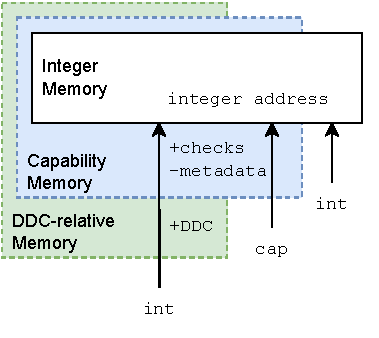
\includegraphics[width=\linewidth]{Figures/cheri_memory.pdf}
      \captionof{figure}{Emulator memory structure}
      \label{fig:emulatormemory}
    \end{minipage}\hfill%
    \begin{minipage}[c]{7.5cm}
        \centering
        {

        \small
      \begin{algorithmic}
        \If{new CHERI instruction}
            \State handle with \code{XCheri64}
        \ElsIf{basic \code{rv64} instruction}
            \If{in capability encoding mode}
                \State handle with \code{Rv64imCapabilityMode}
            \Else{}
                \State wrap memory with DDC-relative
                \State handle with \code{Rv64im}
            \EndIf{}
        \ElsIf{vector instruction}
            \If{in capability encoding mode}
                \State handle with vector unit
            \Else{}
                \State wrap memory in DDC-relative
                \State handle with vector unit
            \EndIf{}
        % \ElsIf{CSR instruction}
        %     \State handle with CSR module
        \EndIf{}
    \end{algorithmic}
        }
    \captionof{figure}{Example algorithm for emulating \code{rv64imvxcheri}}\label{fig:module_algorithm}
    \end{minipage}
\end{figure}

The capability model presented by the C/Rust library has one flaw.\label{safetaggedcap}
Each \code{CcxCap} instance stores capability metadata (e.g. the uncompressed bounds) as well as the compressed encoding.
This makes it potentially error-prone to represent untagged integer data with \code{CcxCap}, as the compressed and uncompressed data may not be kept in sync and cause inconsistencies later down the line.
\code{CcxCap} also provides a simple interface to set the tag bit, without checking whether that is valid.
The emulator introduced the \code{SafeTaggedCap} to resolve this: a sum type which represents either a \code{CcxCap} with the tag bit set, or raw data with the tag bit unset.
This adds type safety, as the Rust compiler forces every usage of \code{SafeTaggedCap} to consider both options, preventing raw data from being interpreted as a capability by accident and enforcing Provenance.

% i.e. doing capability relocation
The final hurdle was the capability relocations outlined in \cref{chap:bg:subsec:cherirelocs}.
Because we're emulating a bare-metal platform, there is no operating system to do this step for us.
A bare-metal C function has been written to perform the relocations\footnote{\gitfile{src/crt_init_globals.c}{CTSRD-CHERI/device-model}{https://github.com/CTSRD-CHERI/device-model/blob/88e5e8e744d57b88b0dbb8e3456ee0e69afc143b/src/crt_init_globals.c}}, which could be compiled into the emulated program.
We decided it would be quicker to implement this in the simulator, but
in the future we should be able to perform the relocations entirely in bare-metal C.

\subsection{Emulating vectors}
% i.e. using addr, provenance split to write agnostic code?

Vector instructions are executed by a Vector ISA module, which stores all registers and other state.
\code{VLEN} is hardcoded as 128-bits, chosen because it's the largest integer primitive provided by Rust that's large enough to hold a capability.
\code{ELEN} is also 128-bits, which isn't supported by the specification, but is required for capabilities-in-vectors (\cref{chap:capinvec}).
Scaling \code{VLEN} and \code{ELEN} any higher would require the creation and integration of new types that were more than 128-bits long.

To support both CHERI and non-CHERI execution pointers are separated into an address and a \emph{provenance}\footnote{The ``original allocation the pointer is derived from''\cite{memarianExploringSemanticsPointer2019}, or in CHERI terms the bounds within which the pointer is valid.}.
The vector unit retrieves an address + provenance pair from the base register, generates a stream of addresses to access, then rejoins each address with the provenance to access memory.
When using capabilities, provenance is defined in terms of the base register e.g. \enquote{the provenance is provided by capability register X}, or defined by the DDC in integer mode\footnote{See \cref{chap:emu:rvv_int_mode} for the reasoning behind this decision.}.
On non-CHERI platforms the vector unit doesn't check provenance.

Arithmetic and configuration instructions are generally simple to implement, so aren't covered here.
The emulator splits vector memory accesses into three phases: decoding, checking, and execution.
A separate decoding stage may technically not be necessary in hardware (especially the parts checking for errors and reserved instruction encodings, which a hardware platform could simply assume won't happen), but it allows each memory access instruction to be classified into one of the five archetypes outlined in \cref{chap:bg:sec:rvvmemory}.
It is then easy to define the checking and execution phases separately for each archetype, as the hardware would need to do.

\subsubsection{Decoding phase}\label{chap:hardware:subsec:decoding}
Decoding is split into two steps: finding the encoded \paramt{nf} and \paramt{eew} values, then interpreting them based on the encoded archetype.
% Vector memory accesses are encoded under the F extension's Load and Store major opcodes, which already encodes an element width.
Vector memory access instructions are encoded similarly to the F extension's floating-point load/store instructions, which include an ``element width''.
The vector extension adds four extra ``element width'' values which imply the access is vectorized.
% This element width is used to differentiate between vector accesses and scalar floating-point accesses, where a vector access can have one of four widths (8, 16, 32, 64).
If any of these values are found, the instruction is interpreted as a vector access and \paramt{nf} is extracted.
% \paramt{nf} is encoded consistently in all vector memory access instructions

Once the generic parameters are extracted, the \paramt{mop} is checked to determine the indexing method (Unit, Strided, Indexed-Ordered, or Indexed-Unordered).
If a unit access is selected, the second argument field encodes an extra value to choose between different unit-stride archetypes (normal unit access, fault-only-first, whole register, or bytemask).
Strided and indexed accesses just use their dedicated archetypes.
Once the archetype is found, supplemental calculations can be performed (e.g. computing \code{EVL = ceil(vl/8)} for bytemask accesses), and the relevant information is returned as a \code{DecodedMemOp} enumeration.

\todomark{diagram of floating point ld/st vs. vector ld/st}
\todomark{Decision tree for operation decoding}

\subsubsection{Fast-path checking phase}\label{chap:hardware:subsec:checking}
The initial motivation for this project was investigating the impact of capability checks on performance.
We investigate an approach using a \enquote{fast-path}, where certain instructions could check their whole access range against a capability immediately rather than check each individual element.
Other approaches, such as optimizing a parallel checker for $n$ elements, were too hardware-specific and couldn't be modelled in software as well.
\cref{chap:hardware:sec:fastpath} describes methods for calculating the \enquote{tight bounds} for each access type, i.e. the minimum range of bytes that must be accessible, and ways that architectural complexity can be traded off to calculate \emph{wider} bounds.

The emulator calculates tight bounds for all accesses.
If this bounds doesn't pass the capability check, the emulator raises an imprecise trap and stops immediately.
In the case of fault-only-first loads, where synchronous exceptions (e.g. capability checks) are explicitly handled, the access continues regardless and elements are checked individually.
This is also the expected behaviour if a capability check for \emph{wider} bounds fails.
The emulator deviates from the spec in that \code{vstart} is \emph{not} set when the tight bounds check fails, as it does not know exactly which element would have triggered the exception.
As noted in \cref{chap:hardware:sec:fastpath}, a fully compliant machine must check each access to find \code{vstart} in these cases.

\subsubsection{Execution phase}\label{chap:hardware:subsec:execution}
If the fast-path check deems it appropriate, the emulator continues execution of the instruction in two phases.
First, the mapping of vector elements to accessed memory addresses is found.
The code for this step is independent of the access direction, and an effective description of how each type of access works.
It can be found in \todomark{appendix XYZ}.
The previously computed tight bounds are sanity-checked against these accesses, and the accesses are actually performed.

\subsubsection{Integer vs. Capability encoding mode\label{chap:emu:rvv_int_mode}}
As noted in \cref{chap:bg:subsec:cheriencodingmode} CHERI-RISC-V defines two execution modes that the program can switch between.
In Integer mode \enquote{address operands to existing RISC-V load and store opcodes contain integer addresses} which are implicitly dereferenced relative to the default data capability, and in Capability mode those opcodes are modified to use capability operands.
Integer mode was included in the interests of maintaining compatibility with legacy code that hasn't been adapted to capabilities.
As similar vector code may also exist, CHERI-RVV treats vector memory access instructions as \enquote{existing RISC-V load and store opcodes} and requires that they respect integer/capability mode.
\section{Fast-path calculations\label{chap:hardware:sec:fastpath}}
Because CHERI, and indeed the vector extension, target all levels of computer architecture from embedded systems to cloud servers, it's important for fast-paths to be scalable and adjust to the implementation complexity.
To that end, we propose a method of generating the address range for accesses of each archetype, noting where architectural complexity can be traded off for tighter coverage.

\todomark{fast-path could be split up? i.e. for LMUL = 8, could execute a fast-path for each register in the group rather than all 8 at once}

\subsection{Possible fast-path outcomes}
In some cases, a failed address range check may not mean the access fails.
The obvious case is fault-only-first loads, where capability exceptions may be handled without triggering a trap.
Implementations may also choose to calculate wider bounds for the sake of simplicity, or even forego a fast-path check altogether.
Thus, a fast-path check can have three outcomes depending on the circumstances:
\begin{itemize}
    \item Success - All accesses will succeed
    \item Likely-Failure - At least one access \emph{may} raise an exception
    \item Failure - At least one access \emph{must} raise an exception
    \item Unchecked
\end{itemize}

\todomark{if an address range is calculated then: if capability contains it: SUCCESS else if it was wide or FoF: Likely-Failure else: FAILURE}
\todomark{if an address range isn't calculated: Unchecked}
\todomark{Put the above into an algorithm format}

A Success means no per-access capability checks are required.
Likely-Failure and Unchecked results mean each access must be checked, to see if any of them actually raise an exception.
Unfortunately, accesses still need to be checked under Failure, because both precise and imprecise traps need to report the offending element in \code{vstart}\footnote{In very particular cases, e.g. unmasked unit-strided accesses where \code{nf = 1}, the capability bounds could be used to calculate what the offending element must have been. We believe this is too niche of a use case to investigate further, particularly given the complexity of the resulting hardware.}.

Because all archetypes may have Failure or Likely-Failure outcomes, hardware must provide a fallback slow-path for each archetype which checks/performs each access in turn.
In theory, a CHERI-RVV specification could relax the \code{vstart} requirement for imprecise traps, and state that all capability exceptions trigger imprecise traps.
In this case, only archetypes that produce Likely-Failure outcomes need the slow-path.
However, it is likely that for complexity reasons all masked accesses will use wide ranges, thus producing Likely-Failure outcomes and requiring slow-paths for all archetypes anyway.
Because the Likely-Failure and Failure cases require the slow-path anyway, computing the fast-path can only be worthwhile if Success is the common case.

\newcommand{\vstart}{\code{vstart}}
\newcommand{\vstartactive}{\code{vstart}_{\mathit{active}}}
\newcommand{\evl}{\code{evl}}
\newcommand{\evlactive}{\code{evl}_{\mathit{active}}}
\newcommand{\baseaddr}{\mathit{base}}

\subsection{Masked accesses}
For all masked accesses, masked-out/inactive segments should not trigger capability exceptions.
Therefore, a tight bounds must include only the smallest and largest active segments.
These segments can be found by inspecting the mask vector: either checking each bit in turn or using parallel logic to find the lowest/highest set bits.
Care must be taken with these checks to ensure elements outside the range $[\textit{vstart}, \textit{evl})$ are not counted.

\begin{align}
    \vstartactive{} &= \min(i\ \forall\ \vstart{} \le i < \evl{}\ \text{where}\ \mathit{mask}[i] = 1) \\
    \evlactive{}    &= \max(i\ \forall\ \vstart{} \le i < \evl{}\ \text{where}\ \mathit{mask}[i] = 1) + 1
\end{align}

\subsubsection*{Tradeoffs}
If using parallel logic to find the lowest/highest bits, it could be difficult to account for $[\textit{vstart}, \textit{evl})$.
An implementation could choose to only calculate tight bounds when the mask is fully utilized, i.e. $\textit{vstart} = 0, \textit{evl} = \textit{VLEN}$, and assume wider bounds otherwise.

Accounting for masked accesses at all may not be worth the extra complexity.
Only elements masked off on the edges make any difference, and it may be uncommon for long runs of edge elements to be masked off.
Thus, an implementation could choose to ignore masking entirely when computing the ranges.
This does mean that all failures become Likely-Failure when masking is enabled, because all elements outside the capability bounds may be masked off.

\todomark{iterating over elements may still be more energy-efficient than doing individual capability checks?}

\subsection{Unit accesses}
For unit segmented accesses, which includes fault-only first, the tight address range for an access is simple to calculate.
Whole register and bytemask accesses can simplify this by fixing \code{nf = 1} and \code{eew = 8}.

\begin{equation}
    \baseaddr{} + [\vstartactive{} * \code{nf} * \code{eew}, \evlactive{} * \code{nf} * \code{eew})
\end{equation}
\todomark{Note that the equation is a simplification of strided for \code{stride = nf * eew}}

\subsubsection*{Tradeoffs}
\code{nf} is not guaranteed to be a power of two (except for the whole-register case), so calculating the `tight' address range would require a multiplication by an arbitrary four-bit value between 1 and 8.
If this multiplication is too expensive, implementations could choose to classify all $\code{nf} > 1$ cases as Unchecked.
% \todomark{if nf == 1; as normal; if nf != 1 Unchecked}

Unless extra restrictions are placed on \code{vstart}, calculating the start of this range requires another arbitrary multiplication.
To avoid this one could assume \code{vstart = 0} and treat failures as Likely-Failure for other cases.
%for the calculation, perform the capability check and treat failures as Likely-Failure (because the failure could be due to an element before \code{vstart}).
% \todomark{make it clear that in this case vstart = 0 would still be a complete failure}
Once could also classify all nonzero \code{vstart} accesses as Unchecked.
% \todomark{if vstart == 0 failure = failure; if vstart != 0 all = Likely-Failure}

Even if the previous two optimizations are applied, the final range still requires a multiplication $\evl{} * \code{eew}$.
Thankfully, because \code{eew} may only be one of four powers-of-two, this can be encoded as a simple shift.

\subsection{Strided accesses}
Strided accesses bring further complication, especially as the stride may be negative.

\begin{equation}
\mathit{bounds}(\code{stride}) = \baseaddr{} + \left\{
    \begin{array}{ll}
          [\vstartactive{} * \code{stride}, (\evlactive{} - 1) * \code{stride} + \code{nf} * \code{eew}) & \code{stride} \ge 0 \\
          
          [(\evlactive{} - 1) * \code{stride}, \vstartactive{} * \code{stride} + \code{nf} * \code{eew}) & \code{stride} < 0
    \end{array} 
\right.
\end{equation}

This is formed of three components:
\begin{itemize}
    \item $\vstartactive{} * \code{stride}$, the start of the first segment. This can be simplified to 0, just like for unit accesses, to avoid an arbitrary multiplication.
    \item $(\evlactive{} - 1) * \code{stride}$, the start of the final segment. This requires an arbitrary multiplication, unless strided accesses are all Unchecked.
    \item $\code{nf} * \code{eew}$, the length of a segment, which can be implemented with a shift.
\end{itemize}
% Because the stride is not guaranteed to be larger than a segment (or even larger than a single element)

% \todomark{stride may be negative}

\subsection{Indexed accesses}
This is the most complicated access of the bunch, because the addresses cannot be computed without reading the index register.

\begin{align}
    [&\baseaddr{}\ +\ \min(\code{offsets}[\vstartactive{}..\evlactive{}]), \\
    &\baseaddr{}\ +\ \max(\code{offsets}[\vstartactive{}..\evlactive{}])\ +\ \code{nf} * \code{eew})
\end{align}

The most expensive components here are of course $min,\,max$ of the offsets.
These could be calculated in hardware through parallel reductions, making it slightly more efficient than looping over each element.
A low-hanging optimization could be to remove the $\vstartactive{}..\evlactive{}$ range condition, performing the reduction over the whole register group, which would make failures Likely-Failure where $\vstartactive{}\ !=\ 0\ ||\ \evlactive{}\ !=\ \code{VLMAX}$.
This calculation could also be restricted to certain register configurations to reduce the amount of required hardware.
Indeed, the amount of hardware could be reduced to zero by simply classifying all indexed accesses as Unchecked.
\section{Going beyond the emulator}
The emulator is a single example of a conformant CHERI-RVV implementation, and does not exercise every part of the specification.
Four properties stand out:
\begin{itemize}
    \item The emulator assumes all element accesses are naturally aligned, but the spec allows misaligned accesses.
    \item The emulator doesn't consider multiple hardware threads, essentially assuming all accesses are atomic.
    \item Segments/elements are always accessed in order, despite the spec not enforcing ordering
    \item Imprecise traps are used for all exceptions - precise trap behaviour is not explored.
\end{itemize}
This section notes how relaxed access ordering and precise exceptions may affect the hardware in ways not previously explored.

\subsection{Misaligned accesses}
Implementations are allowed to handle vector accesses that are not aligned to the size of the element.
This support is independent of misaligned scalar access support, so if e.g. misaligned 64-bit scalar accesses are allowed, misaligned vector accesses of 64-bit elements do \emph{not} have to be allowed.

Changing the emulator to allow misaligned accesses of integer data would not have any impact on CHERI correctness.
Capability loads/stores must be aligned to \code{CLEN}\cite[Section 3.5.2]{TR-951}, and an implementation cannot change this.
Writing misaligned integer values across a \code{CLEN} boundary would need to make sure to zero the tag bit on both regions, but this applies to scalar implementations as much as vector ones.
Alignment only impacts CHERI-RVV to the extent that it impacts capabilities-in-vectors (\todoref{capinvec - alignment requirements}).

\subsection{Atomicity of accesses/General memory model}
Vector memory instructions are specified to follow the RISC-V Weak Memory Ordering model\todocite{RVV}\footnote{Behaviour under the Total Store Ordering extension hasn't been defined.}, although this model hasn't been fully explained in terms of vectors yet.
RVWMO defines a global order of \enquote{memory operations}: atomic operations that are either loads, stores, or both\todocite[Chapter 14]{RISCV spec}.
The RVWMO spec assumes all memory instructions create exactly one memory operation but calls out that once the vector model is formalized, vector accesses may be defined to create multiple operations.

The RVV spec states \enquote{vector misaligned memory accesses follow the same rules for atomicity as scalar misaligned memory accesses}, i.e. that misaligned accesses may be decomposed into multiple memory operations of any granularity\footnote{e.g. each byte could be written in a separate access.}.
This is the only mention of atomicity in that document.

Again, atomicity of integer data doesn't really impact the fusion of CHERI and RVV, as long as tag bits are correctly zeroed on all integer writes.
However, it does impact capabilities-in-vectors (\todoref{capinvec - atomicity}).

\subsection{Relaxed access ordering and precise traps}
Ordering is only enforced insofar as it is observable.
The only instructions that are forced to perform their accesses in order are indexed-ordered accesses, which can be used to write to e.g. I/O regions where order matters, and instructions that trigger precise traps.
Precise traps require \code{vstart} to be set to a value such that all elements before \code{vstart} have completed their accesses, and all accesses on/after \code{vstart} have not completed or are idempotent.

If a vector memory access instruction is 1. not indexed-ordered and 2. guaranteed not to trigger a precise trap\footnote{Even instructions that \emph{would} trigger precise traps but are guaranteed not to throw an exception or respond to asynchronous interrupt may execute out of order.} then it may execute out of order.
This does not affect CHERI-RVV in any way.
\section{Testing hypotheses}

\hypsubsection{hyp:hw_cap_as_vec_mem_ref}{Feasibility}
This is true.
All vector memory access instructions index the scalar general-purpose register file to read the base address, and CHERI-RVV implementations can simply use this index for the scalar capability register file instead.
This can be considered through the lens of adding CHERI to any RISC-V processor, and in particular adding Capability mode to adjust the behaviour of legacy instructions.
RVV instructions can have their behaviour adjusted in exactly the same way as the scalar memory access instructions.

That approach then scales to other base architectures that have CHERI variants.
For example, Morello's scalar Arm instructions were modified to use CHERI capabilities as memory references\cite[Section 1.3]{armltdMorelloArchitectureReference2021}, so one may simply try to apply those modifications to e.g. Arm SVE instructions.
This only works where Arm SVE accesses memory references in the same way as scalar Arm instructions did i.e. through a scalar register file.

Arm SVE has some addressing modes like \code{u64base}, which uses a vector as a set of 64-bit integer addresses\cite{armltdArmCompilerScalable2019}.
This has more complications, because simply dereferencing integer addresses without a capability is insecure.
Would a CHERI version convert this mode to use capabilities-in-vectors, breaking compatibility with legacy code that expects integer references?
Another option would be to only enable this instruction in Integer mode, and dereference relative to the DDC.
It's possible to port this to CHERI, but requires further investigation and thought.

\hypsubsection{hyp:hw_cap_bounds_checks_amortized}{Fast-path checks}
This is also true, at least for Successful accesses.
Because the RVV spec requires that the faulting element is \emph{always} recorded\cite[Section 17]{specification-RVV-v1.0}, a Failure due to a capability violation requires elements to be checked individually.
CHERI-RVV could change the specification so the faulting element doesn't need to be calculated, which would make Failures faster, but that still requires Likely-Failures to take the slow-path.

There are many ways to combine the checks for a set of vector elements, which can take advantage of the range constraints.
For example, a unit-stride access could a hierarchy of checks: cache-line checks until a Likely-Failure, then tight $m$-element bounds until a Likely-Failure, then the slow-path.
However, the choice of fast-path checks is inherently a trade-off between latency, area, energy usage, and more.
Picking the right one for the job is highly dependent on the existing implementation, and indeed an implementation may decide that parallel per-element checks is better than a fast-path.


\end{document}